%%=============================================================================
%% Prototype
%%=============================================================================

\chapter{Prototype}
\label{ch:prototype}

\section{Inleiding}

In dit hoofdstuk zal binnen het bestaande platform Innerdreams gamification worden geïmplementeerd, gebruik makend van DNN. Er werd gekozen om een puntensysteem, een badgesysteem, een scorebord en een beloningswinkel te implementeren. Deze elementen werden gekozen na een brainstormsessie en een kort onderzoek over de verschillende manieren waarop gamification kan worden geïmplementeerd.

\section{Gamification binnen Innerdreams}

Zoals hierboven werd vermeld, zal gamification worden geïmplementeerd. Gebruikers kunnen punten verzamelen door enquêtes in te vullen en te delen. Meer specifiek kunnen punten worden verzameld per ingevulde pagina van de enquête, per volledig ingevulde enquête, per gedeelde enquête en per gedeelde enquête die ingevuld werd. Ook kunnen gebruikers badges verzamelen als ze een mijlpaal hebben bereikt en zal een scorebord worden weergegeven met daarop de personen met het hoogste aantal punten. De verzamelde punten kunnen worden gebruikt om verschillende artikelen aan te schaffen in de beloningswinkel.

\section{Punten}

Om het puntensysteem uit te werken werd gekozen om gebruikers punten te laten verzamelen bij het invullen en delen van enquêtes. Hiervoor is het nodig om de mogelijkheid te bieden om aan bepaalde enquêtes punten te gaan toewijzen.
 
Een eerste noodzakelijke aanpassing was het toevoegen van een tabel aan de SQL databank om de punten hierin bij te houden. Zoals te zien is in Figuur \ref{fig:dbdiagram} bestaat de tabel uit de volgende kolommen:

\begin{itemize}
    \item PuntenID: de primaire sleutel als unieke identificatie
    \item Pagina: het aantal punten dat wordt verdiend bij het volledig invullen van een pagina van een enquête.
    \item EnqueteCompleted: het aantal punten dat wordt verdiend bij het volledig voltooien van een enquête.
    \item Share: het aantal punten dat wordt verdiend bij het delen van een enquête.
    \item ShareCompleted: het aantal punten dat wordt verdiend bij het succesvol voltooien van een enquête door de persoon met wie de enquête is gedeeld.
    \item EnqueteID: de vreemde sleutel die de punten linkt aan een enquête.
\end{itemize}

\begin{figure}
    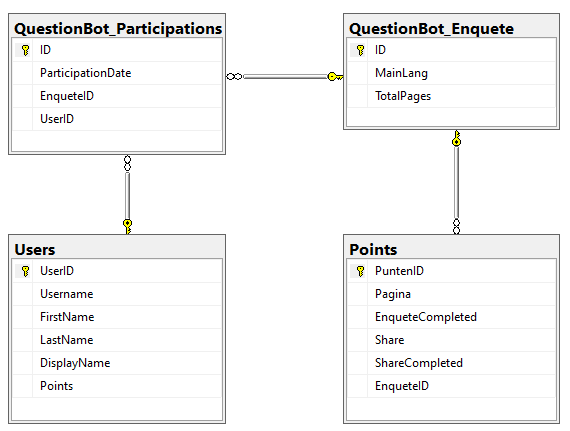
\includegraphics[width=\linewidth]{DBDiagram.png}
    \caption{Het model van de punten.}
    \label{fig:dbdiagram}
\end{figure}

Het was ook nodig om het totale aantal verzamelde punten van iedere individuele gebruiker bij te houden. In Figuur \ref{fig:dbdiagram} is te zien dat aan de gebruikerstabel een extra kolom werd toegevoegd om deze punten te linken aan de gebruikers. Voor zowel nieuwe gebruikers als de reeds bestaande werd de standaard waarde van hun punten op nul gezet.

Om de punten effectief toe te wijzen aan de verschillende enquêtes werd een nieuwe module, die te zien is in Figuur \ref{fig:managepoints}, aangemaakt. In deze module worden de bestaande enquêtes opgehaald en kunnen door de beheerder de respectievelijke punten worden toegewezen.

\begin{figure}
    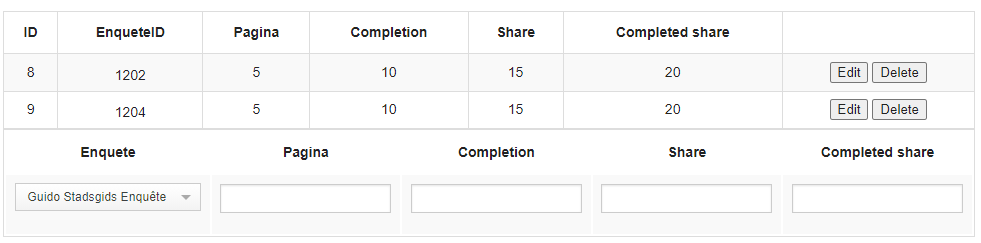
\includegraphics[width=\linewidth]{ManagePoints.png}
    \caption{De beheertool om punten toe te wijzen.}
    \label{fig:managepoints}
\end{figure}

Om een overzicht te geven van het totaal aantal verzamelde punten tijdens het afleggen van een enquête werd ook een overzichtspagina toegevoegd. Als een enquête geen punten heeft toegewezen gekregen zal een korte bedanking worden getoond op dit overzicht. Deze pagina verschijnt eenmaal een gebruiker een enquête volledig heeft ingevuld. Op deze pagina is het ook mogelijk om de huidige enquête te gaan delen met anderen, waardoor nog meer punten kunnen worden verdiend.

Het is soms ook mogelijk dat een gebruiker niet moet aangemeld zijn om een enquête in te vullen. Om te zorgen dat de verzamelde punten niet verloren gaan worden deze bijgehouden in zogenaamde sessievariabelen. Een sessievariabele is een object dat voor elke gebruiker apart wordt bijgehouden op de server zolang een sessie tussen de gebruiker en de server actief is. De totale waarde van de verzamelde punten wordt bijgehouden in een sessievariabele tijdens het afleggen van een enquête. Eenmaal de gebruiker op de overzichtspagina terechtkomt en hij/zij is niet aangemeld wordt de optie gegeven om zich alsnog aan te melden. Als de gebruiker vervolgens aangemeld is zal terug worden doorverwezen naar de overzichtspagina waar de gebruiker de verzamelde punten, bijgehouden in de sessievariabele, kan verzilveren.

Als een enquête wordt gedeeld zal deze een aantal extra parameters bevatten in de URL, waaronder een uniek cijfer dat de gebruiker die de enquête gedeeld heeft zal identificeren. Bij het starten met het afleggen van een enquête wordt een controle uitgevoerd op de URL. Als deze URL de eerder vermelde unieke identificatie bevat zullen aan deze gebruiker een aantal vooraf vastgelegde punten worden toegewezen. Eenmaal de enquête wordt voltooid zullen opnieuw aan deze gebruiker een aantal punten worden toegewezen.

\section{Badges}

Voor het behalen van badges werd gekozen om deze te koppelen aan het totale aantal deelnames van een gebruiker aan enquêtes. Eenmaal een gebruiker tenminste één pagina heeft ingevuld zal een deelname aan deze enquête worden toegevoegd aan de databank.

In Figuur \ref{fig:dbbadge} is te zien dat een tabel voor het bijhouden van de verschillende badges werd toegevoegd aan de SQL databank. Deze tabel bestaat uit de volgende kolommen:

\begin{itemize}
    \item ID: de primaire sleutel als unieke identificatie
    \item ImageLink: een verwijzing naar de afbeelding van de badge.
    \item Title: een titel die de badge beschrijft.
    \item TriggerQuery: een SQL-query die wordt uitgevoerd eenmaal aan een bepaalde voorwaarde voldaan is.
\end{itemize}

\begin{figure}
    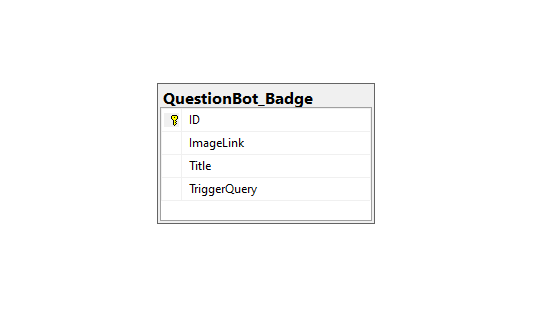
\includegraphics[width=\linewidth]{DBBadge2.png}
    \caption{De badge tabel.}
    \label{fig:dbbadge}
\end{figure}

Wanneer een gebruiker op de overzichtspagina van de enquête terechtkomt zullen twee lijsten van badges opgehaald worden. De eerste lijst van badges bestaat uit alle badges die in het systeem zitten. De tweede lijst van badges omvat alle behaalde badges van de gebruiker. Deze twee lijsten worden met elkaar vergeleken en als een badge wordt tegengekomen die de gebruiker nog niet heeft behaald zal worden gecontroleerd of hij/zij aan de voorwaarden voor het behalen ervan voldoet. Deze controle gebeurt aan de hand van het uitvoeren van een stored procedure, die te zien is in Listing \ref{lst:csb}. Binnen deze stored procedure zal de eerder vernoemde trigger query die gelinkt is aan de desbetreffende badge worden uitgevoerd.

\begin{lstlisting}[caption={De CheckSucceededBadge stored procedure.},
    label={lst:csb},
    language=SQL,
    showspaces=false,
    basicstyle=\ttfamily,
    numbers=left,
    numberstyle=\tiny,
    numbersep=1pt,
    breaklines=true
    commentstyle=\color{gray}]
    ALTER PROCEDURE [dbo].[QuestionBot_CheckSucceededBadge](@BadgeID int, @UserID int) as
    BEGIN
    Declare @statement as nvarchar(max) 
    set @statement = (select TriggerQuery from QuestionBot_Badge where ID = @BadgeID) 
    EXECUTE sp_executesql @statement , N'@UserID int',@UserID=@UserID
    END
\end{lstlisting}

In Listing \ref{lst:tq} is te zien hoe zo een trigger query er uit ziet. Voor een gebruiker wordt de som van zijn/haar totale aantal deelnames aan alle enquêtes genomen. Als deze som voldoet aan een bepaalde voorwaarde zal het cijfer 1 worden geretourneerd, wat wil zeggen dat de gebruiker een badge heeft behaald. Als 0 wordt geretourneerd wil dit zeggen dat niet aan de voorwaarde is voldaan. In dit voorbeeld is te zien dat voor de huidige gebruiker wordt gecontroleerd of hij/zij minstens één enquête heeft voltooid. Als aan deze voorwaarde voldaan is zal deze persoon een badge verdienen met bijvoorbeeld de tekst ``Vul je eerste enquête in''.

\begin{lstlisting}[caption={De badge trigger query.},
    label={lst:tq},
    language=SQL,
    showspaces=false,
    basicstyle=\ttfamily,
    numbers=left,
    numberstyle=\tiny,
    numbersep=1pt,
    breaklines=true
    commentstyle=\color{gray}]
    declare @Participations int set @Participations = (select count(*) from QuestionBot_Participations where UserID = @UserID) 
    if (@Participations >= 1) select 1 else select 0
\end{lstlisting}

\section{Scorebord}

Het scorebord werd ontworpen om respectievelijk de rangschikking, de gebruikersnaam en het totale aantal verzamelde punten van alle gebruikers weer te geven. In dit geval was het niet nodig om aanpassingen te doen aan de databank aangezien alle noodzakelijke wijzigingen reeds werden uitgevoerd in de vorige stappen.

Om alle benodige data van de gebruikers op te halen werd de volgende stored procedure gebruikt, te zien in Listing \ref{lst:gul}. Hierin wordt gebruik gemaakt van de \textit{SQL ROW\_NUMBER()} functie. Deze functie wijst aan elke rij uit de resultatenlijst een unieke, oplopende waarde toe op basis van een geordende lijst. Hier zal deze functie op basis van de oplopende lijst van punten van gebruikers een waarde toewijzen die de rangschikking op het scorebord zal voorstellen. Als in de lijst twee gelijke waarden voor de punten worden tegengekomen zal de waarde worden toegewezen op basis van de alfabetische volgorde van de gebruikersnamen. Buiten het ophalen van de rangschikking zal deze stored procedure ook de gebruikersnamen en punten ophalen van alle gebruikers.

\begin{lstlisting}[caption={De GetUsersLeaderboard stored procedure.},
    label={lst:gul},
    language=SQL,
    showspaces=false,
    basicstyle=\ttfamily,
    numbers=left,
    numberstyle=\tiny,
    numbersep=1pt,
    breaklines=true
    commentstyle=\color{gray}]
    ALTER procedure [dbo].[GetUsersLeaderboard] as
    select ROW_NUMBER() OVER(ORDER BY Points desc, DisplayName) as Rank, DisplayName, Points from dbo.Users
    where IsSuperUser = 0
\end{lstlisting}

De opgehaalde data wordt in een overzichtelijke tabel weergegeven, te zien in Figuur \ref{fig:leaderboardinnerdreams}. Binnen deze tabel kan worden gesorteerd en gefilterd. Er kan gesorteerd worden op zowel de rangschikking, de gebruikersnaam als het aantal behaalde punten en er kan gefilterd worden op de gebruikersnaam. De tabel zal initieel alle gebruikers weergeven maar de keuze kan ook gemaakt worden om enkel de top vijf van alle gebruikers met het meeste aantal punten weer te geven.

\begin{figure}
    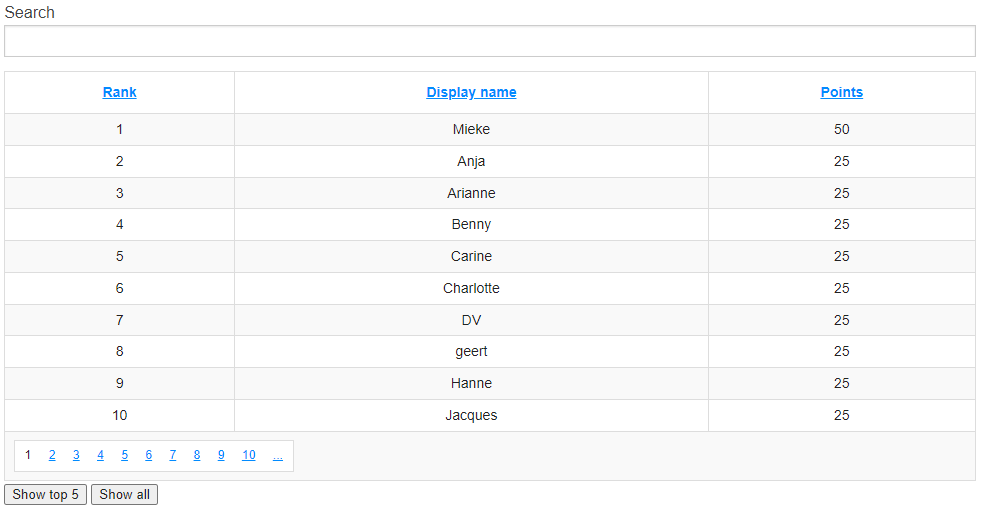
\includegraphics[width=\linewidth]{LeaderboardInnerdreams.png}
    \caption{Het scorebord op Innerdreams.}
    \label{fig:leaderboardinnerdreams}
\end{figure}

\section{Beloningswinkel}


